\section{Numerische Verfahren}

\subsection{Fehler}

\begin{tabular}{ll}
Tatsächlicher Wert \quad  & $\phi(t_n)$ \\
Globaler Fehler & $E_n = \smash{\displaystyle\max_{0 \leq k \leq n}} \lvert e_k \rvert = \smash{\displaystyle\max_{0 \leq k \leq n}}\lvert x(t_k) - x_k\rvert$ \\ \\
Lokaler Fehler & $\tau_{k,h} = \frac{x(t_{k+1}) - x_h(t_{k+1}; t_k, x(t_k))}{h}$ \\
Rundungsfehler & $R_n = y_n - Y_n$\, ,\quad wobei $Y_n$ gerundet \\
Lipschitz-Bedingung & $\lvert f(t, x_1) - f(t, x_2)\rvert \leq L \lvert x_1 - x_2 \rvert$ wobei $\dot{x} = f(t,x), L = const.$ \\
\end{tabular}\\ \\
Zwei Lösungen $x^{(1)}(t), x^{(2)}(t)$ bezüglich der Anfangsbedingungen $x_1, x_2$. Dann gilt für alle $t$ in einer Umgebung von $t_0$ die Abschätzung: $\lvert x^{(1)}(t) - x^{(2)}(t)\rvert \leq e^{L(t-t_0)} \lvert x_1 - x_2\rvert $ \newline

\begin{minipage}{0.6\linewidth}
    \subsection{Explizites Euler-Verfahren (Polygonzugmethode)}
    Polygonzug mit Steigung $y'(t)$ und Zeitschritt $h$\\
    $\dot{x} = f(t,x)$ \\
    $t_k = t_0 + k \cdot h$ \\
    $x_{k+1} = x_k + h \cdot f(t_k, x_k)$ \\
    $x_0 = x(0)$ \\
    $|\phi''(t)|<M \qquad |e_n| < \dfrac{M*h^2}{2} \qquad
    h_n < \sqrt{\dfrac{2\epsilon}{M}} \qquad E_n \approx h$\\
    $e_{n+1} = \dfrac{1}{2} \cdot \varphi''(\tau_n)\cdot h^2 \qquad \tau_n \text{ zwischenschritt in } [t_n,t_{n+1}]$\\
    $\varphi''(t)=f_t(t,\varphi(t)) + f_y(t,\varphi(t))\cdot\varphi'(t)$\\\\
\end{minipage}
\begin{minipage}{0.4\linewidth}
  %  \centering
    \begin{tikzpicture}

\begin{axis} [
    clip=false,
    width=8cm, height=4cm,
    axis lines=left,
    domain=-2:2, samples=31,
    ymin=0, ymax=6,
    xmin=-2, xmax=3,
    xticklabels={{},{},{$t_0$},{$t_1$},{$t_2$},{$t_3$},{}},
    yticklabels={},
]
    \node at (axis cs:3.2,0) {$t$};
    \node at (axis cs:-2,6.5) {$y$};
    
    % Plot parabola
    \addplot[HSRBlue,mark=none] {4-0.5*x^2};
    \addplot[HSRBlue,mark=o,only marks,samples=3,domain=-1:1] {4-0.5*x^2};
    
    % p0
    \addplot[black,mark=none,domain=-1.5:-0.5,samples=2] {4.5+x};
    \node[anchor=south] at (axis cs:-1,3.5) {$p_0$};
    \addplot[black,dashed,mark=none,domain=-0.5:0,samples=2] {4.5+x};

    % p1
    \addplot[black,mark=none,domain=-0.5:0.5,samples=2] {4.5};
    \node[anchor=south] at (axis cs:0,4.5) {$p_1$};
    \addplot[black,mark=o] coordinates{(0,4.5)};
    \addplot[black,dashed,mark=none,domain=0.5:1,samples=2] {4.5};
    
    % p2
    \addplot[black,mark=none,domain=0.5:1.5,samples=2] {5.5-x};
    \node[anchor=south] at (axis cs:1,4.5) {$p_2$};
    \addplot[black,mark=o] coordinates{(1,4.5)};
    \addplot[black,dashed,mark=none,domain=1.5:2,samples=2] {5.5-x};
    
    % p3
    \node[anchor=south] at (axis cs:2,3.5) {$p_3$};
    \addplot[black,mark=o] coordinates{(2,3.5)};
    
\end{axis}

\end{tikzpicture}
\end{minipage} 

\begin{minipage}{0.6\linewidth}
    \subsection{Mittelpunktsregel, Polygonzugmethode}
     Modifiziertes Euler-Verfahren mit Schätzung in der Mitte. \\
     $t_k = t_0 + k \cdot h$ \\
     $x_{k+\frac{1}{2}} = x_k + \frac{h}{2} \cdot f(t_k, x_k)$ \\
     $x_{k+1} = x_k + h \cdot f(t_k + \frac{h}{2}, x_{k+\frac{1}{2}})$ \\
\end{minipage}
\begin{minipage}{0.4\linewidth}
   % \centering
	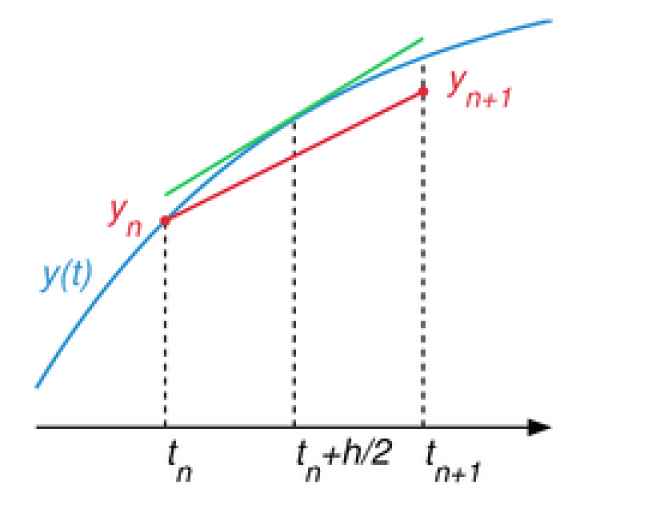
\includegraphics[width= 0.6\textwidth]{images/mittelpunkt.png}
\end{minipage}
\begin{minipage}{0.6\linewidth}
    \subsection{Heun-Verfahren}
    Trapez Approximation \\
    $t_k = t_0 + k  \cdot h$ \\
    $x_0 = x(0)$ \\
    $m_1 = f(t_k, x_k)$ \\
    $m_2 = f(t_k + h, x_k + hm_1)$\\
    $x_{k+1} = x_k + \frac{h}{2}(m_1 + m_1)$\\
    $e_n  \approx h^3 \qquad E_n \approx h^2$\\
\end{minipage}
\begin{minipage}{0.4\linewidth}
   % \centering
    \begin{tikzpicture}

\begin{axis} [
    clip=false,
    width=6cm, height=5cm,
    axis lines=left,
    domain=0:2.5,samples=31,
    xmin=-0.5, xmax=3.5,
    ymin=0, ymax=6,
    xticklabels={{},{},{$t_{i-1}$},{$t_i$},{}},
    yticklabels={{},{},{$f(t_{i-1},\varphi_{i-1})$},{$f(t_i,\varphi_i)$},{}},
]
    
    % Plot parabola
    \addplot[HSRBlue,mark=none] {x^2};
    \addplot[HSRBlue,mark=o,only marks] coordinates {(1,1)(2,4)};

    % Euler
    \addplot[HSRHematite,mark=none,fill=HSRHematite80,fill opacity=0.2] coordinates {(1,0)(1,1)(2,1)(2,0)(1,0)};
    \draw[HSRHematite] (axis cs:1.8,0.6) -- (axis cs:2.2,0.8) node[anchor=west] {$I_{\text{Euler}}$};    
    
    % Heun
    \addplot[HSRReed,mark=none,fill=HSRReed80,fill opacity=0.2] coordinates {(1,0)(1,1)(2,4)(2,0)(1,0)};
    \draw[HSRReed] (axis cs:1.8,2) -- (axis cs:2.2,2.2) node[anchor=west] {$I_{\text{Heun}}$};
    
\end{axis}

\end{tikzpicture}
\end{minipage}
\begin{minipage}{0.6\linewidth}
    \subsection{Runge-Kutta}
    $t_k = t_0 + k \cdot h$ \\
    $x_0 = x(0)$ \\
    $m_1 = f(t_k, x_k)$\\
    $m_2 = f(t_k + \frac{h}{2}, x_k + \frac{h}{2} m_1)$ \\
    $m_3 = f(t_k + \frac{h}{2}, x_k + \frac{h}{2} m_2)$ \\
    $m_4 = f(t_k + h, x_k + hm_3)$ \\
    $x_{k+1} = x_k + \frac{h}{6} \left(m_1 + 2m_2 + 2m_3 + m_4\right)$ \\
    $e_n \approx h^5 \qquad E_n \approx h^4$
\end{minipage}
\begin{minipage}{0.4\linewidth}
%	\centering
	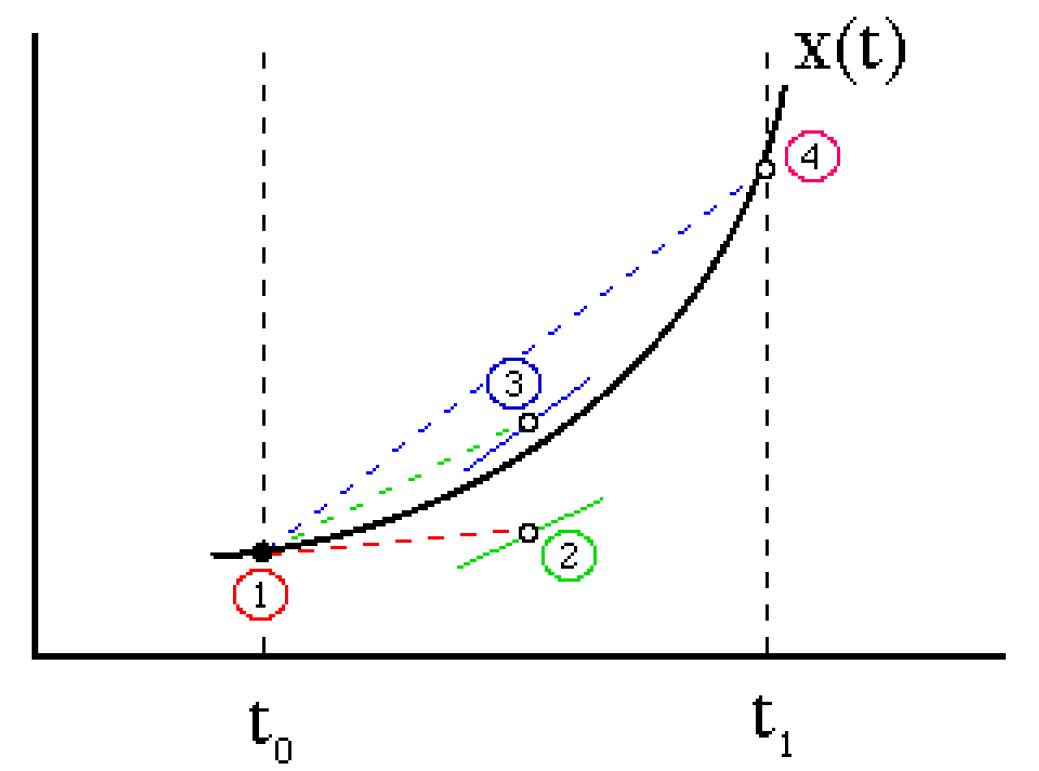
\includegraphics[width= 0.7\textwidth]{images/RK4.png}
\end{minipage}